\subsection{EEG Signal Processing \& Entropy}
In general, there are two approaches to analyze EEG signal:  (i) a spatio-temporal method, mainly guided by the detection of event-related potentials (ERPs), and (ii) spectral analysis. The former appears too sensitive to be reliably used in a consistent way with a single-channel dry consumer-grade EEG, such as the Neurosky Mindwave \cite{}. To account for dynamics of brain synchronization in the spectral domain, every 0.25 second we analyze the frequency domain $0-128Hz$ (the hardware sampling rate is 512 Hz), by computing the power spectrum density associated with the Fourier transform of the signal over each period. Figure \ref{fig:pspectrum} shows typical power spectrum densities, associated with simple tasks, such as {\it resting state} (i.e. closed eyes, no mental focus) \cite{}, {\it passively watch a screen (with a video?)}, and read a text in English on the same screen, in silence and loud. We see that the structure of the power spectrum density varies significantly across tasks. This result is consistent also across subjects \textcolor{red}{[\bf bring evidence here.]}.

 \begin{figure}[!t]
\centering
%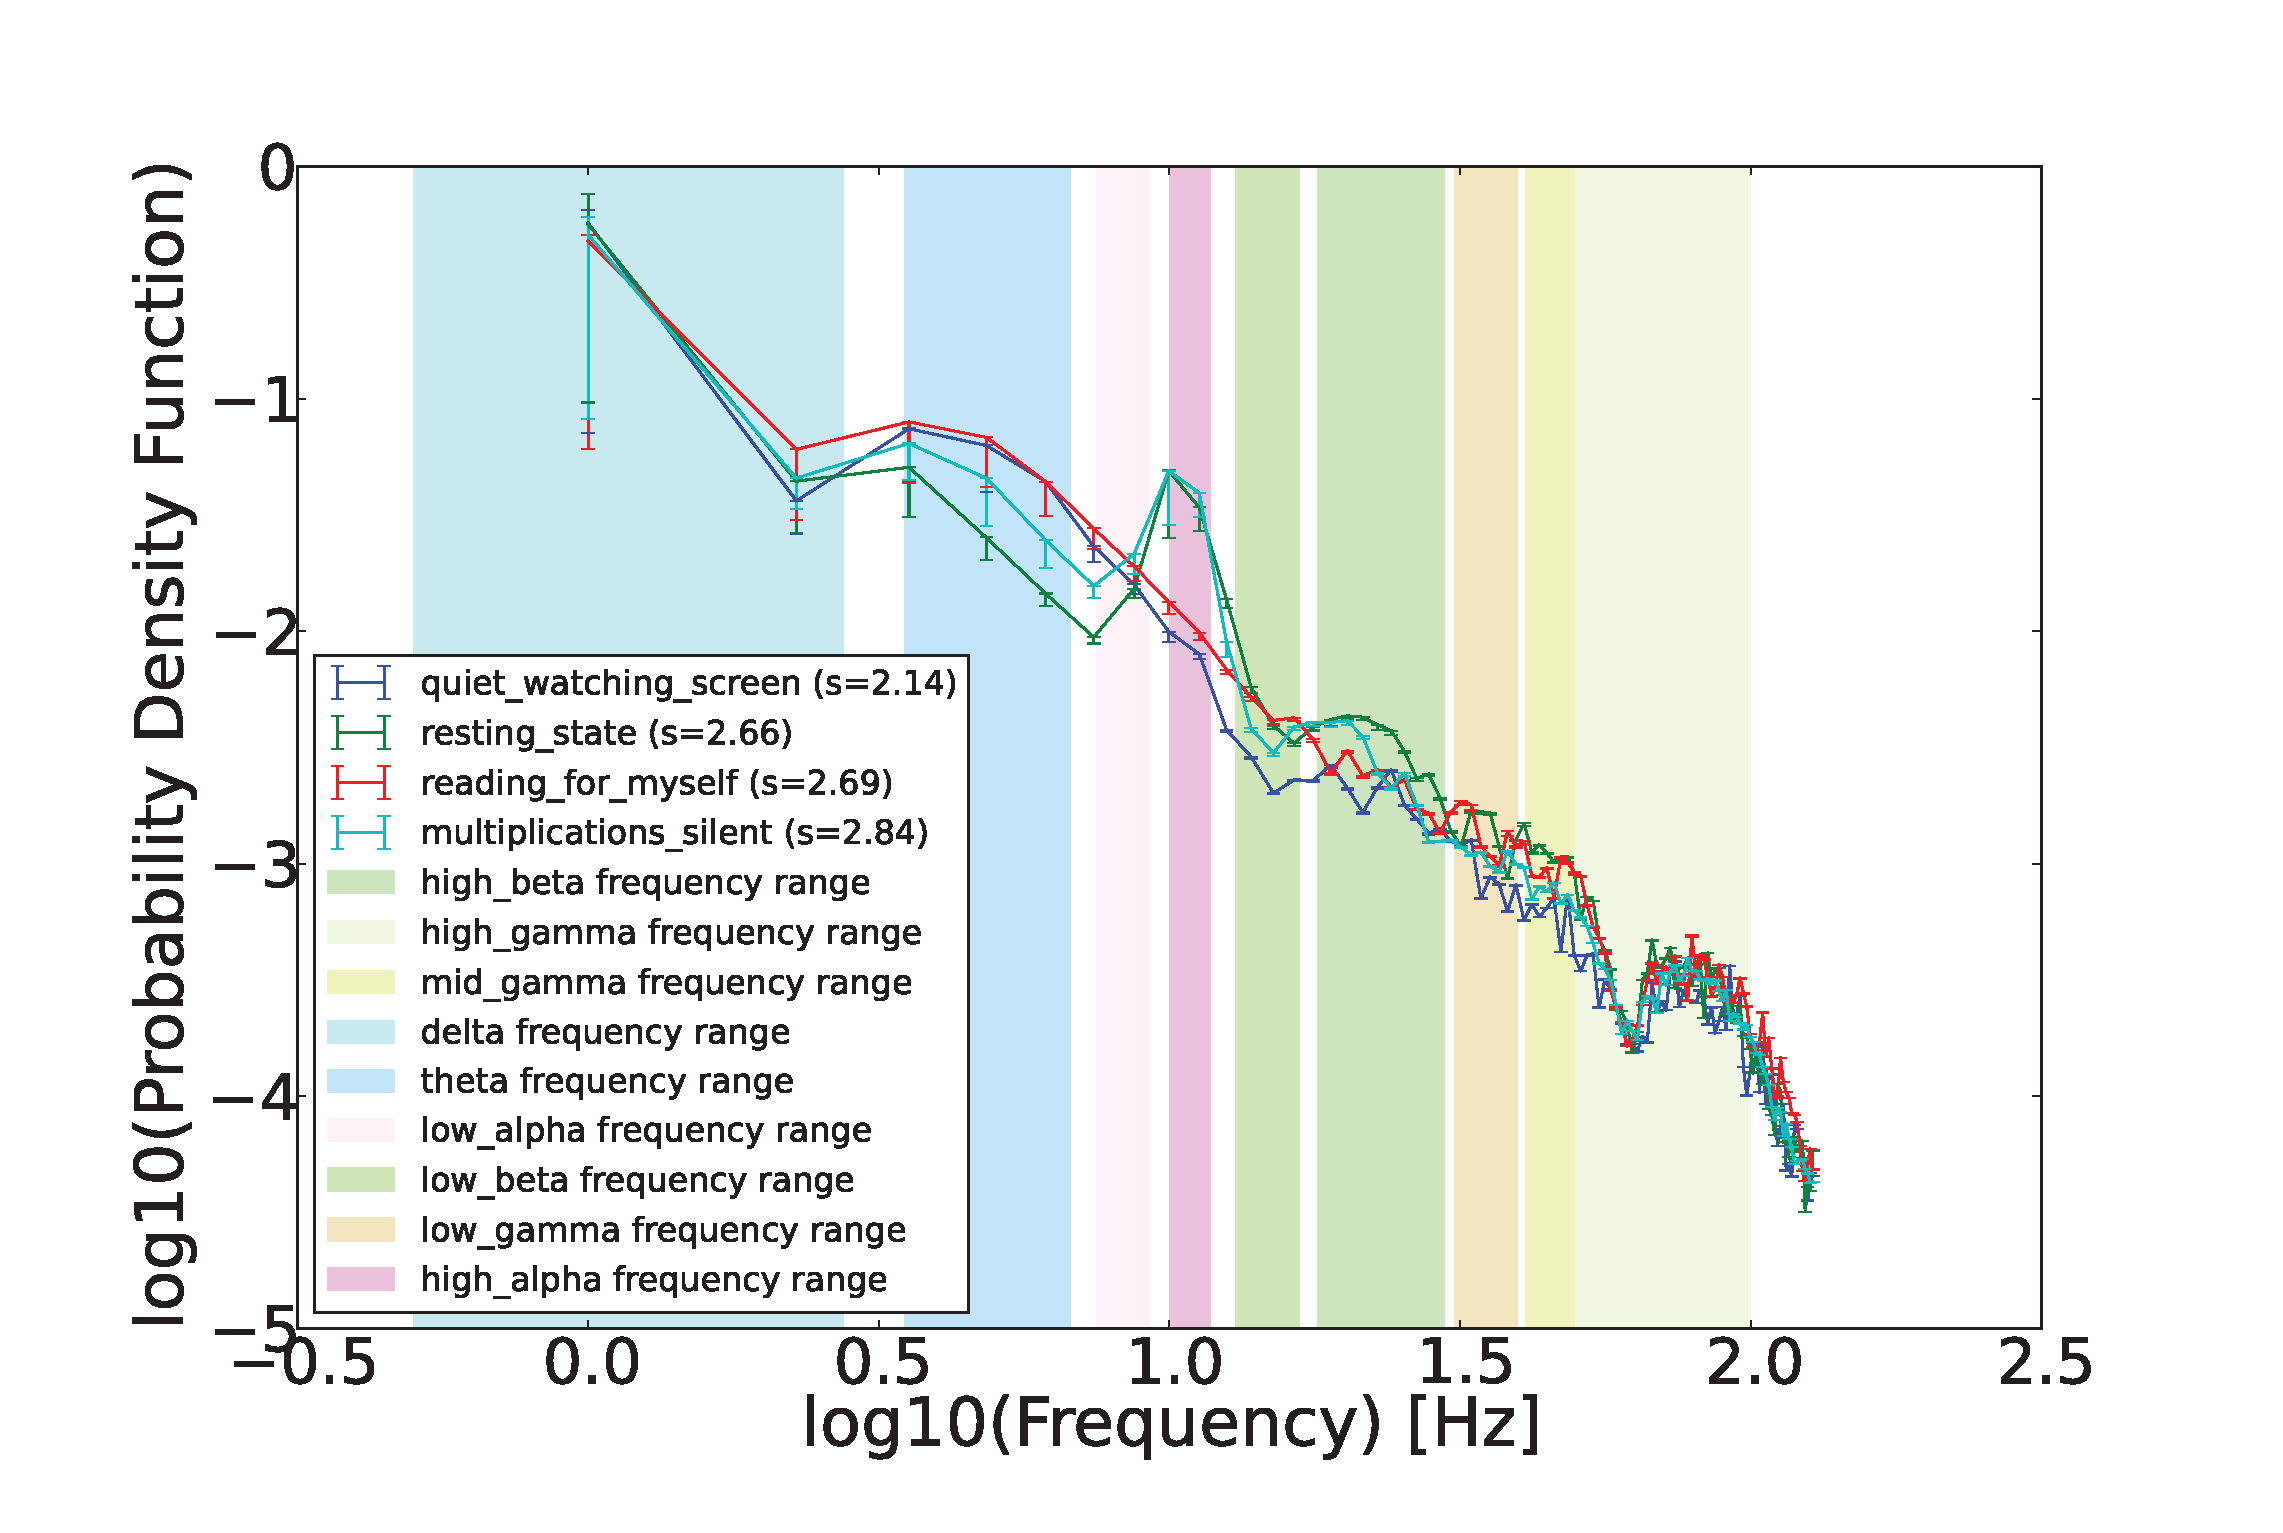
\includegraphics[width=1.1\columnwidth]{../figures/compareArtifacts.eps}
\caption{Show the difference between resting state, being passive in front of a screen, and actively reading a text, in double logarithmic scale.}
\label{fig:pspectrum}
\end{figure}

Figure \ref{fig:pspectrum} shows the heavy-tailed distribution of the power spectrum density, approximately a straight line in double logarithmic scale, which corresponds to current understanding of the pink noise nature of brain synchronization, $pdf(f) \sim 1/f^{\mu+1}$, with $f$ the frequency and $\mu \approx 1$ \cite{pink noise brain}.

From previous research, we know that the density of the power spectrum increases in case of increased cognitive activity \cite{}, in particular in the case of reading a text, which is of interest here \cite{}. 

Entropy is one simple and non-parametric way to account for the variation of power spectrum density function$pdf(f)$. The simplest and most common entropy metric is the one of Boltzmann for any logarithmic base, or more specifically the entropy of Shannon in base 2, given by,

%\begin{equation}
%\label{eq:tsallis}
%S_q(X) = \frac{1}{q-1} \left[ 1 - \sum_{i=1}^n (p_i)^q \right].
%\end{equation}

\begin{equation}
\label{eq:shannon}
S = - \sum_{i=1}^n p_i\cdot log_{2}(p_i).
\end{equation}

Entropy is a very convenient metric for our purpose, because it represents nothing else than the discrete integral of the logarithmic frequency densities. In other words, it provides a single scalar value, which accounts for all the power spectrum density function $pdf(f)$.\footnote{There are several reasons for not choosing any of the built-in {\it meditation} and {\it attention} metrics provided by Neurosky: (i) these metrics are proprietary, and it is therefore impossible to know what purpose they exactly serve (i.e., what are definitions of meditation and attention according to Neurosky?); (ii) we nevertheless suspect that they take an average of $\alpha$ and $\beta$ frequency ranges as an input, which is more restrictive than our approach, especially given that the ranges of $\alpha$ and $\beta$ frequency may vary from one subject to another when reading \cite{}.} 

Entropy $S$ shall only be seen as a convenient coarse-grained and compressed measure of neural synchronization in the brain over a short period. As we aim to measure variations of synchronization states over time, a relative value of $S$ is accurate. For that, entropy normalized over a short period of time is sufficient to capture short-term variations of neural coherence as a result of cognitive tasks, involving solicitation of short-term memory, and quick recalls of conceptual elements from long-term memory. We therefore define 

\begin{equation}
\label{eq:Snormalized}
S_{norm}(t) = \frac{S(t) - \langle S \rangle}{\sigma_{S}}, 
\end{equation}

with $\langle S \rangle$ and $\sigma_{S}$ the average and standard deviation of the entropy $S$ calculated over the last 20 points (i.e., the last 5 seconds). %By definition, $S_{norm}$ is always centered around $0$.

Like any other measure taking EEG as an input, entropy is subjected to artifacts, in particular eye-blinks. We shall later expose how to reduce, or on the contrary harness, the influence of non-neural artifacts recorded by the EEG. Nevertheless, EEG entropy offers therefore a non-parametric way to compress information contained in the power spectrum density into a single scalar instantaneous value. Normalized entropy $S_{norm}$ ensures that only local variations are captured. 

%We wanted a lightweight mobile apparatus, which does not require complicated machine learning or any communication with a cloud service, or would not drain a battery. We purposely decided for a cheap update method {\bf [continue this point in discussion because it helps introduce future work]}
